% !TEX root = tracking.tex
\section{General Framework \label{sec:framework}}
Details of the framework are summarized in Figs. \ref{fig:fw_offline}, \ref{fig:fw_online}, and \ref{fig:hybrid_ctrl}. 
%\subsection{Offline Framework}
The purpose of the offline framework (Fig. \ref{fig:fw_offline}) is to generate a TEB and corresponding optimal tracking controller that can be quickly and easily used by the online framework.
%To determine both the TEB and optimal tracking controller functions/look-up tables, an offline framework is used as shown in Fig. \ref{fig:fw_offline}. 
The planning and tracking model dynamics are used in the reachability precomputation (described in sec. \ref{sec:precomp}), whose solution is a value function that acts as the TEB function/look-up table. 
The gradients of the value function comprise the optimal tracking controller function/look-up table. 
These functions are independent of the online computations and environment -- they depend only on the \textit{relative system state} and dynamics between the planning and tracking models, not on absolute states along the trajectory at execution time.

\begin{figure}[h!]
	\centering
	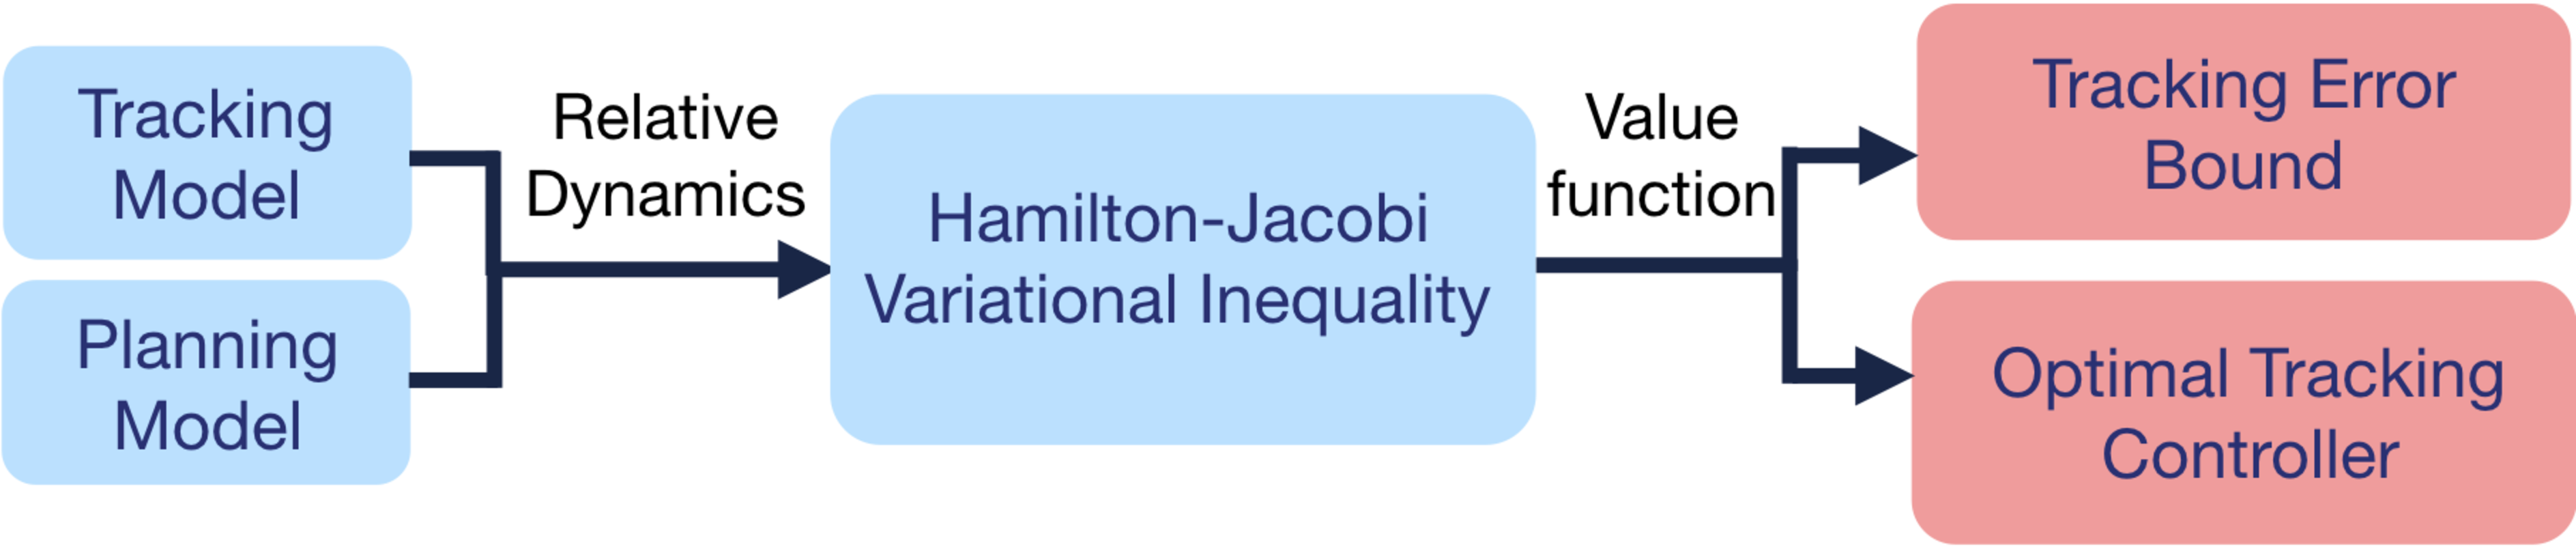
\includegraphics[width=1\columnwidth]{fig/framework_offline_2}
	\caption{Offline framework. Output of offline framework shown in red.}
	\label{fig:fw_offline}
\end{figure}

%\subsection{Online Framework}
Online, we start in the bottom-left corner of Fig. \ref{fig:fw_online} to determine the tracking model's initial state (i.e. autonomous system's initial state). Based on this we initialize the planning model such that the tracking model is within the TEB relative to the planning model. The state of the planning model is entered into a planning algorithm.  
\begin{figure}[h!]
	\centering
	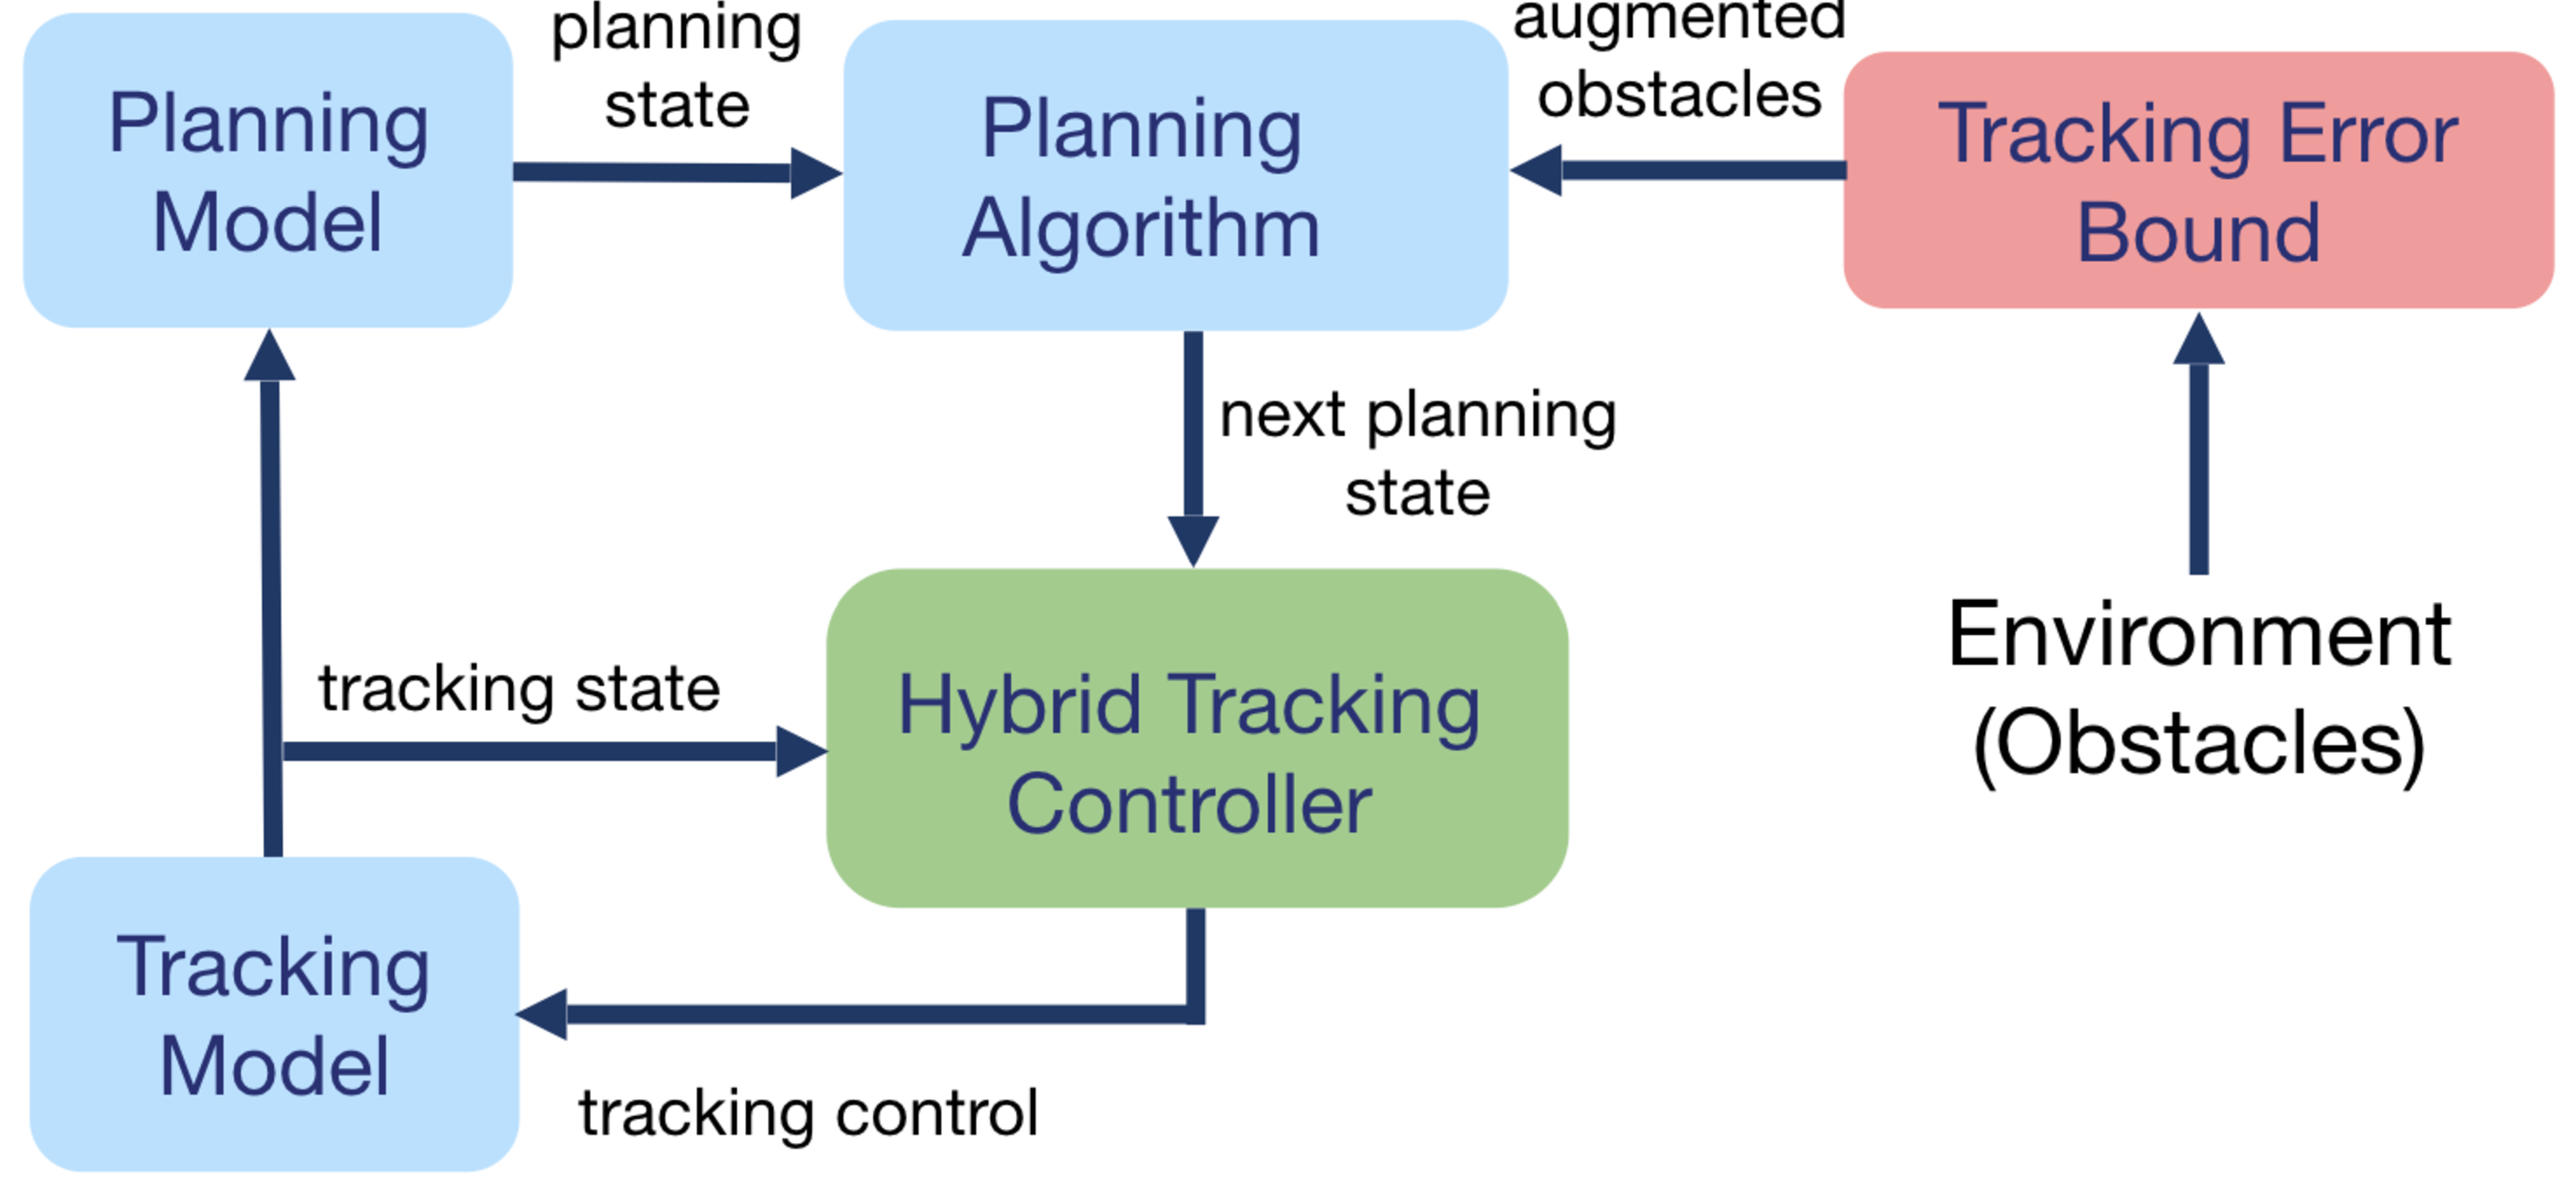
\includegraphics[width=1\columnwidth]{fig/framework_online_2}
	\caption{Online framework. Components from offline computation shown in red.}
	\label{fig:fw_online}
\end{figure}
Another input to the planning algorithm is the set of augmented constraints $\constrAug$.  These are acquired by updating constraints $\constr$ and accordingly updating the sensed constraints $\constrSense$ in the environment.  This can be done, for example, by sensing the environment for obstacles. Next, $\constrSense$ is augmented  by the precomputed TEB using the Minkowski difference to produce the augmented constraints $\constrAug$. \footnote{for a faster method of augmenting obstacles we typically simply expand each obstacle by the maximum distance of the TEB in each dimension for a conservative approximation}
%; our framework is agnostic to the planing algorithm, so any may be used. 
%We will present three example using planning algorithms FSM, RRT, and MPC in Section \ref{sec:results}.



%This TEB can be thought of as a ``safety margin'' that guarantees robustness despite the worst-case disturbance and planning model evolution. 
In terms of obstacles in the environment, augmenting the constraints by this margin can be thought of as equivalent to wrapping the planning model of the system with a ``safety bubble''. 
The planning algorithm takes in the planning model state and augmented constraints and outputs a next desired state for the planning model towards $\contrgoal$.
%then These augmented constraints are given as inputs to the planning algorithm along with the current state of the planning model of the system. 
%The planning algorithm then outputs the next state of the planning model.
%The tracking model is a more accurate representation of the physical system (such as a quadrotor or a car). 
The hybrid tracking controller block takes in this next planning model state along with the current state of the tracking model.
Based on the relative state between these two models, the hybrid tracking controller outputs a control signal to the autonomous system. 
The goal of this control is to make the autonomous system track the desired planning state as closely as possible.
This cycle continues as the planning algorithm moves towards $\contrgoal$.

%In the context of real-time robust planning towards a target in an unknown environment, we propose a framework for combining fast planning methods that do not need to take into account disturbances, and HJ reachability analysis which provides formal guarantees for systems with disturbances. The high level idea of the framework is summarized in Fig. \ref{fig:fw_online}, \ref{fig:hybrid_ctrl}, and \ref{fig:fw_offline}. Formal definitions will be introduced in \MCnote{Section \ref{}}.

%Fig. \ref{fig:fw_online} shows the online computations under our framework, which uses a hierarchical structure in which a planner plans a path or trajectory for a simple ``virtual system''. Examples of planners include those based on model-predictive control (MPC), rapidly-exploring random tree (RRT), or neural networks; our framework is agnostic to the planner, so any planner can be used. The choice of the virtual system is also flexible, and depends on the requirements of the planner. We will present an example of a virtual system used in conjunction with an RRT planner in \MCnote{Section \ref{}}. The planner outputs a desired ``virtual state'' of the virtual system.

%The ``real system'' is a model of a physical system such as a quadrotor, and a subset of the state variables forms the virtual state of the virtual system. The state of real system and the desired virtual state are inputs to a hybrid tracking controller. Based on these two inputs, the hybrid tracking controller outputs a control signal to the real system. The goal of this control is to make the real system track the desired virtual state as closely as possible. Our concept of tracking error will be defined in \MCnote{Section \ref{}}.

The hybrid tracking controller is expanded in Fig. \ref{fig:hybrid_ctrl} and consists of two controllers: an optimal tracking controller (also referred to as the safety controller) and a performance controller.
In general, there may be multiple safety and performance controllers depending on various factors such as observed size of disturbances, but for simplicity we will just consider one safety and one performance controller in this paper. 
The optimal tracking controller consists of a function (or look-up table) computed offline by solving a HJ variational inequality (VI), and guarantees that the TEB is not violated, despite the worst-case disturbance and worst-case planning control. 
Although the planning model in general does not apply the worst-case planning control, assuming the worst allows us to obtain a \textit{trajectory-independent} TEB and an optimal tracking controller that is guaranteed safe.
Note that the computation of the value function and optimal tracking controller is done offline; during online execution, the table look-up operation is computationally inexpensive. 
\begin{figure}[h!]
	\centering
	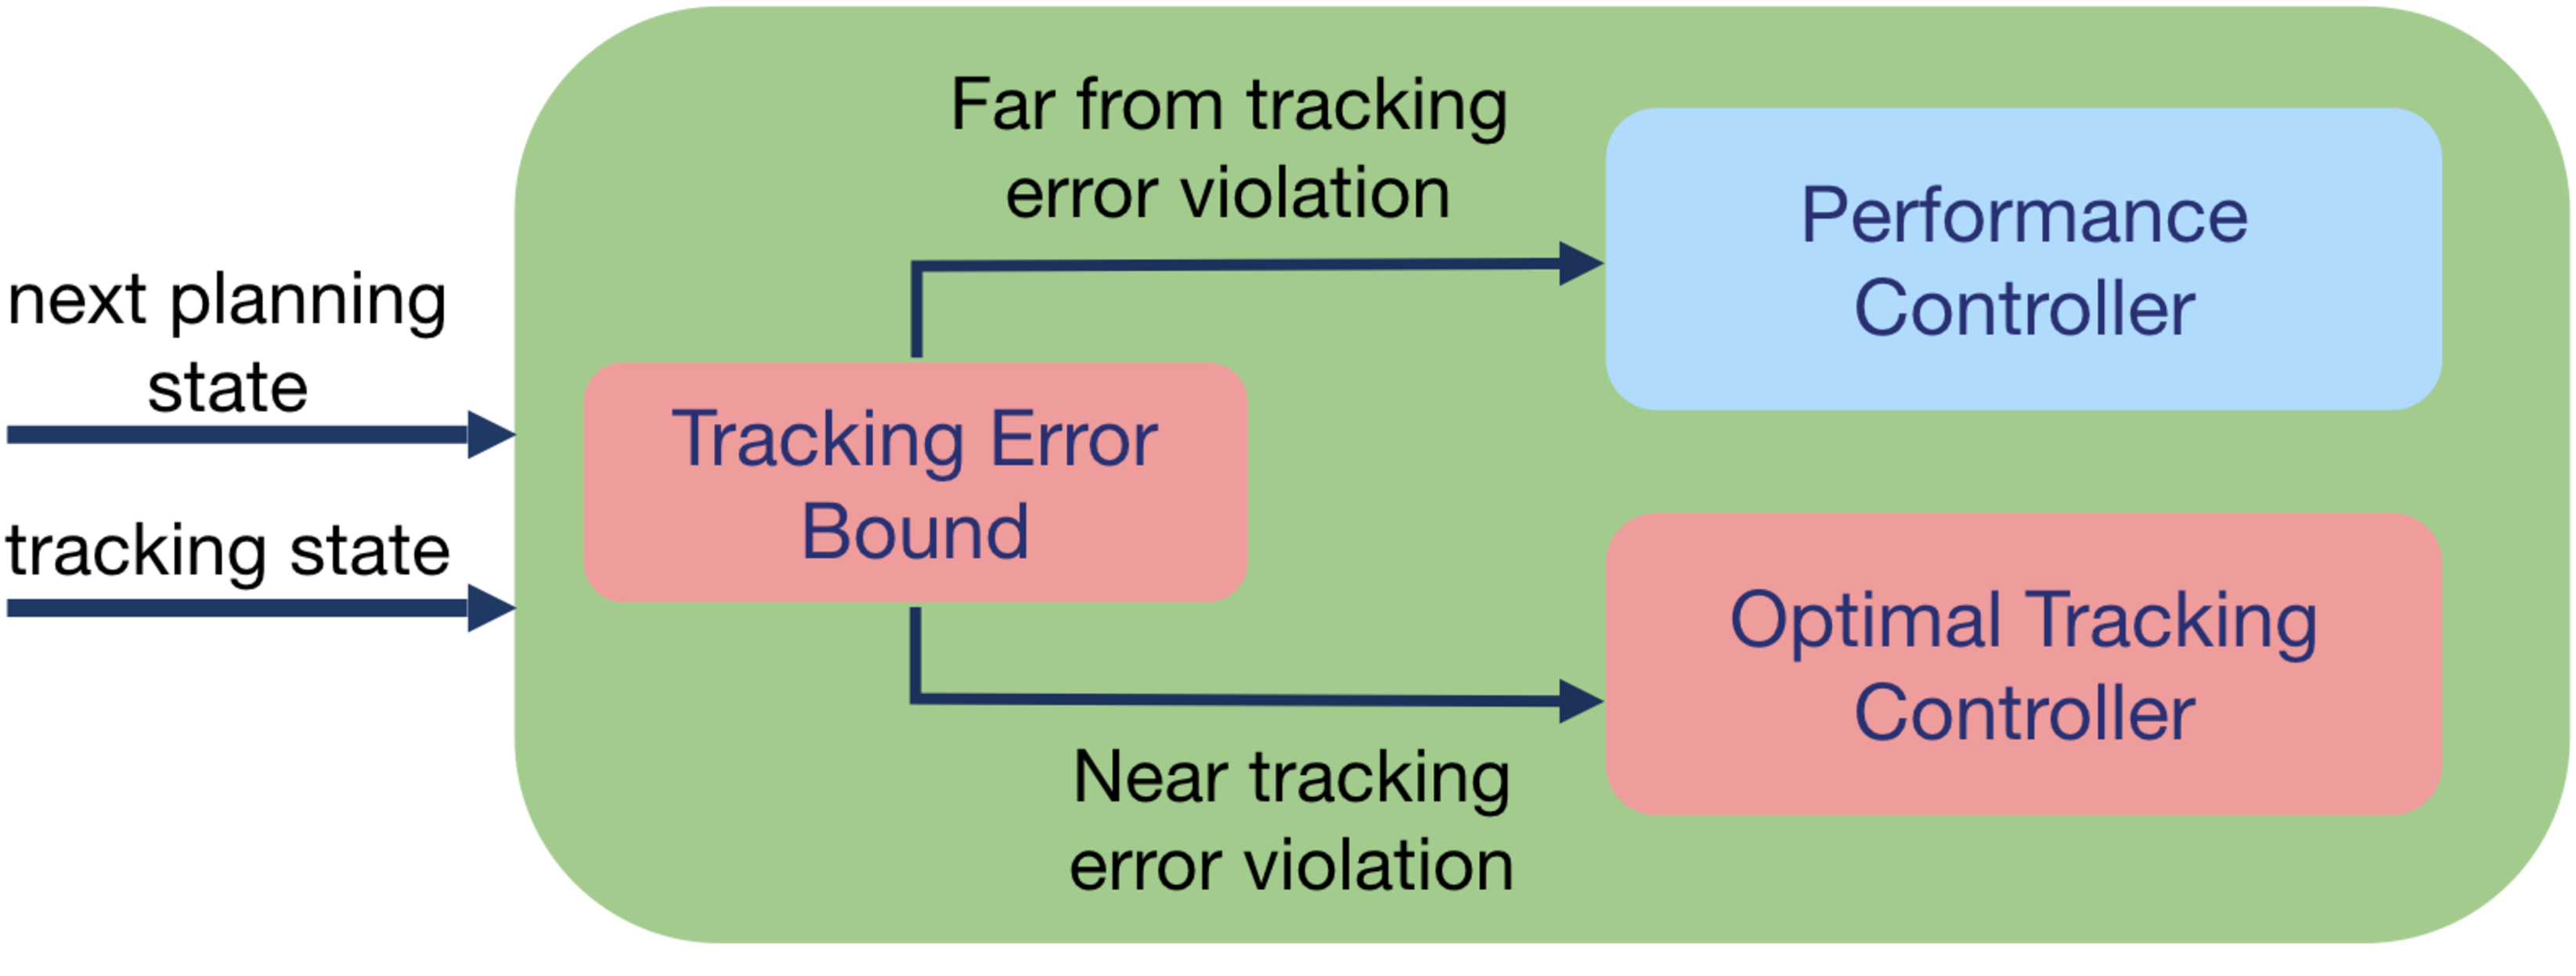
\includegraphics[width=\columnwidth]{fig/hybrid_controller_2}
	\caption{Hybrid controller. Components from offline computation shown in red.}
	\label{fig:hybrid_ctrl}
\end{figure}

When the system is close to violating the TEB, the optimal tracking controller must be used to prevent the violation. 
On the other hand, when the system is far from violating the TEB, any controller (such as one that minimizes fuel usage), can be used. 
This control is used to update the autonomous system, and the process repeats.

In the following sections we will first explain the precomputation steps taken in the offline framework. 
We will then walk through the online framework.
Finally, we will present three numerical examples.

%Besides the virtual state, the planner also takes into account any obstacles that must be avoided. In order to be robust to disturbances, planning must be done with a safety margin that accounts for disturbances. A safety margin that guarantees robustness despite the worst-case disturbance is given by a TEB obtained in the offline HJ reachability computation, shown in Fig. \ref{fig:fw_offline} and explained in detail in \MCnote{Section \ref{}}. The virtual and real system dynamics are used to compute a value function, which simultaneously gives the TEB and the safety controller look-up table used by the hybrid tracking controller.
%
%\textbf{Maybe put next paragraph in the introduction}
%
%There are many fast planners that could potentially do planning in real-time; however, these typically cannot account for disturbances in a provably safe way. In addition, complex system models with nonlinear dynamics complicate planning algorithms (non-convex for MPC, more difficult for RRT). On the other hand, HJ reachability is able to handle disturbances, and is agnostic to system dynamics. In addition, provably guarantees can be provided. However, HJ reachability and in general formal verification methods can be very expensive to compute.
%
%Refer to figure: planning level and safety level. 
%
%In the safety level, we start with the error dynamics, and we compute two things: bubble which is fed into planner to plan with extra margin, and error-feedback controller for real-time control. These two can be computed offline independent of the planned path.
%
%In the planning level, any planning method such as MPC, RRT, etc. (cite some things) can be used. The planning level does not need to take into account disturbances, and can use simple system dynamics or even no dynamics at all. In fact we will be using a simple RRT planner which simply provides paths, in the form of a sequence of line segments, which are not dynamically feasible. 